\documentclass[8pt]{beamer}

\usetheme{Berlin}


\usepackage[noindent]{ctexcap}
\usepackage{graphicx}
%\usepackage{xcolor}
\usepackage{amsmath}
\usepackage{physics}
\usepackage{hyperref}
\usepackage{slashed}
\usepackage{siunitx}

\newcommand{\misE}{\slashed{E}}
\newcommand{\misEt}{\slashed{E}_T}

\title{薛定谔方程中的有效理论和重整化研究}

\author{黄应生}

\institute{山东大学物理学院}
%\institute
%{
%  \inst{1}山东大学
%}

%index:
%section 1:background(4):
%higgs discovery and property
%higgs selfcoupling and higgs pair production
%higgs decay and previous study about higgs pair production
%section 2:signal reconstruction and background rejection
%mainly background, lepton flavour selection(1)
%signal features, signal combination and reconstruction(4)
%mT2,(3)
%mva, results (2)
%section 3: sensivity of lambda_3
%14TeV
%section 4: conclusion and discussion

\begin{document}

\maketitle

\begin{frame}
  \frametitle{目录}
  \tableofcontents
\end{frame}

\section{背景}
\begin{frame}
\frametitle{背景}
\begin{itemize}
  \item 量子场论中的重整化和有效场论
  \vspace{12pt}
  \item 基本思想:舍弃高能态,并用一组新的局域作用项模拟高能态对低能行为的影响
  \vspace{12pt}
  \item 重整化和有效理论的思想也可以运用于量子力学中\footnote{Lepage. How to renormalize the Schr\"odinger equation.Nucl. Th. ,1997.}
\end{itemize}

\end{frame}

\begin{frame}
\frametitle{论文主体内容}
\begin{itemize}
  \item 在非相对论性量子力学中构建一个有效理论
  \vspace{12pt}
  \item 有效理论中的可观测量
  \vspace{12pt}
  \item 有效理论中的矩阵元和波函数
  \vspace{12pt}
  \item 有效理论中微扰论的应用
  \vspace{12pt}
  \item 不同“真实”物理的有效理论
\end{itemize}
\end{frame}

\section{有效理论的构建}
\begin{frame}
\frametitle{“真实”理论}
为方便比较及计算,我们定“真实”理论为
\begin{align}
	H                             & =\frac{\vb{p}^2}{2m}+V(\vb{r}) 
\end{align}
其中$V(\vb{r})=-\dfrac{\alpha}{r}+V_s(\vb{r})$,$V_s(\vb{r})$暂定为
\begin{equation}
  V_s(r)=-\frac{1.04152e^{-0.9991r}}{r}
\end{equation}
这里我们取$\alpha=1$,$m=1$。也即是库伦势加上一个短程势(这里是汤川势)的形式。
\end{frame}

\begin{frame}
\frametitle{有效势的基本形式}
两种尝试:
\begin{itemize}
\item 以$\delta$函数势模拟真实短程作用,但其二阶微扰会出现发散项
\begin{equation}
	V_{app}=-\frac{\alpha}{r}+c\;\delta^3(\vb{r})
\end{equation}
\item 以误差函数模拟真实长程作用,以平滑过的$\delta$函数势($\delta_a^3$)模拟真实短程作用
\begin{align}\label{Veff}
	\nonumber V_{eff} = & -\frac{\alpha}{r}\;\text{erf}(\frac{r}{\sqrt{2}a})+c\; a^2\;\delta_a^3(\vb{r})    \\
	\nonumber           & +d_1\;a^4\;\laplacian{\delta_a^3(\vb{r})}+d_2\;a^4\;\div{\delta_a^3(\vb{r})}\grad \\
	\nonumber           & +\dots                                                                            \\
	\nonumber           & +g\;a^{n+2}\;\grad^n\delta_a^3(\vb{r})                                            \\
	                    & +\dots
\end{align}
\end{itemize}
有效势有无穷多种,这里所列出的仅是一种可能的方法。
\end{frame}

\begin{frame}
\frametitle{得到$V_{eff}$的过程}
新的哈密顿量(仅将原有的势进行替换,成为有效势):
\begin{equation}
	H_{eff}=\frac{\vb{p}^2}{2m}+V_{eff}(\vb{r})
\end{equation}
将库伦势进行傅里叶变换:
\begin{equation*}
	\frac{1}{r}\xrightarrow{F.T.\;\;}\lim_{\varepsilon\rightarrow0}\int_{0}^{\infty}\dd^3r\;\frac{e^{iqr\cos\theta-\varepsilon r}}{r}r^2\sin\theta=\frac{4\pi}{q^2}
\end{equation*}
得到的结果进行截断(乘上$e^{-\frac{q^2a^2}{2}}$)后重新傅里叶变换回坐标空间:
\begin{align*}
	\frac{4\pi}{q^2} & \xrightarrow{\text{cutoff}}\frac{4\pi}{q^2}e^{-\frac{q^2a^2}{2}} \\
	                 & \xrightarrow{F.T.\;\;}\frac{\text{erf}(\frac{r}{\sqrt{2}a})}{r}
\end{align*}
得到$V_{eff}$的首项。
\end{frame}

\begin{frame}
对$\delta$函数同样进行傅里叶变换,并进行截断,得到
\begin{equation}\label{smeardelta}
	\delta_a^3(\vb{r})\equiv\frac{e^{-\frac{r^2}{2a^2}}}{(2\pi)^{\frac{3}{2}}\;a^3}.
\end{equation}
于是我们得到$V_{eff}$的次阶项,这便是我们所谓的平滑过的$\delta$函数。注意到将$V_s$泰勒展开后进行傅里叶变换可得到
\begin{equation}\label{qtaylor}
	v_s(q^2)=v_s(0)+q^2v'_s(0)+\dots
\end{equation}
注意到$v_s(0)$是一个常数,其傅里叶逆变换为一个$\delta$函数,此后以此类推,变换回坐标空间得到
\begin{equation}\label{expand}
	V_s(\vb{r})=c\delta(\vb{r})+d\laplacian{\delta(\vb{r})}+\dots
\end{equation}
将$\delta$函数替换为平滑过的$\delta_a^3$函数,就得到式\eqref{Veff}中的局域修正项(即是除了误差函数项之外的所有项)。这样我们得到式\eqref{Veff}的完整表达式。
\end{frame}

\section{有效理论与“真实”物理的对比}
\begin{frame}
\frametitle{通过相移匹配得到耦合常数}
为使有效理论能够模拟“真实”物理中高能部分对低能物理的影响,我们需要利用“真实”的低能数据与有效理论的低能数据进行匹配已得到耦合常数的值。

我们选用仅有1、2个局域修正项的有效势进行计算:
\begin{align}
	\label{Veffa2}
	V_{eff}^{(a^2)} & =-\frac{\alpha}{r}\;\text{erf}\pqty{\frac{r}{\sqrt{2}a}}+c\; a^2\;\delta_a^3(\vb{r})+\mathcal{O}(a^2)                                                                                  \\
	\label{Veffa4}
	V_{eff}^{(a^4)} & =-\frac{\alpha}{r}\;\text{erf}\pqty{\frac{r}{\sqrt{2}a}}+c\; a^2\;\delta_a^3(\vb{r})+d_1\;a^4\;\laplacian{\delta_a^3(\vb{r})}+d_2\;a^4\;\div{\delta_a^3(\vb{r})}\grad+\mathcal{O}(a^4)
\end{align}
并用低能的物理可观测量对耦合常数进行匹配,这里选用低能S波相移。取截断$a=1$,于是可以求出$V_{eff}^{(a^2)}$中的$ c^{(a^2)}=-44.294$,$V_{eff}^{(a^4)}$中的$c^{(a^4)}=-39.9477$以及${d_1}^{(a^4)}=3.26552$。
\end{frame}
%
%\begin{frame}
%\frametitle{束缚能的对比}
%\begin{figure}[!htbp]
%	\centering
%	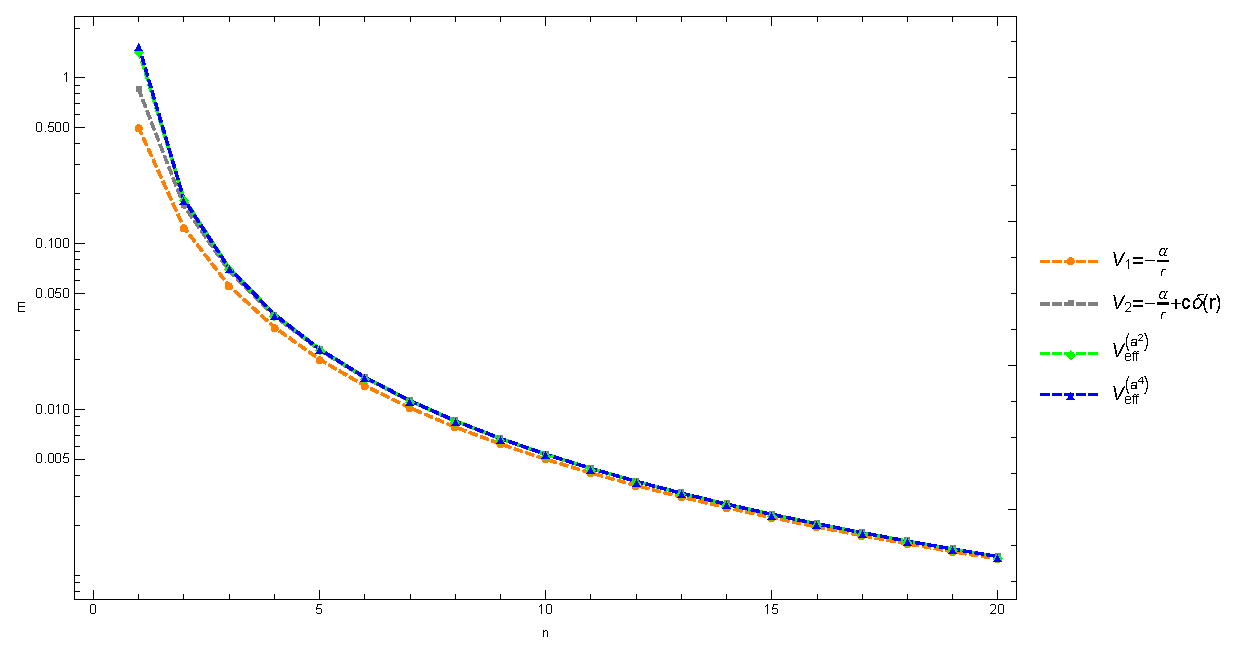
\includegraphics[width=4.3in]{Test_PS_CurveFitting_Figure2_1.eps}
%	\caption{库伦势、$\delta$函数的一阶微扰、$V_{eff}^{(a^2)}$与$V_{eff}^{(a^4)}$的S波束缚能}\label{Swaveenergy}
%\end{figure}
%\end{frame}

\begin{frame}
\frametitle{束缚能误差对比}
\begin{figure}[!htbp]
	\centering
	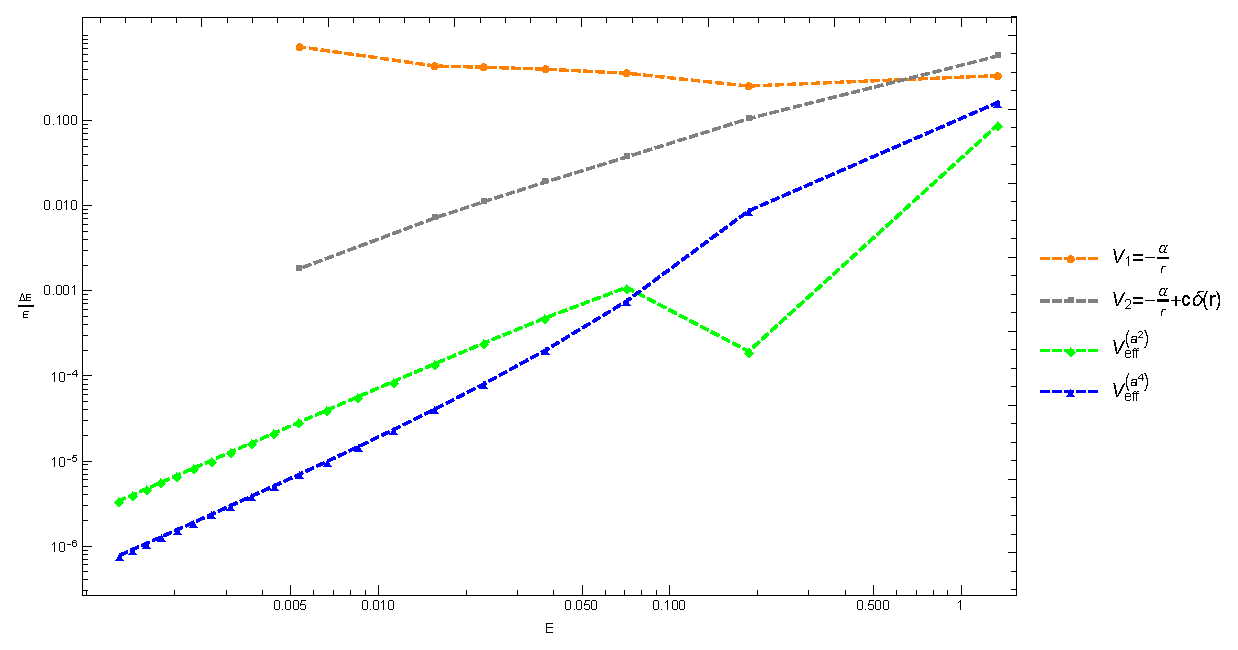
\includegraphics[width=4.3in]{Test_PS_CurveFitting_Figure2.eps}
	\caption{库伦势、$\delta$函数的一阶微扰、$V_{eff}^{(a^2)}$与$V_{eff}^{(a^4)}$相比于“真实”势的S波束缚能相对误差}\label{Swaveenergyerror}
\end{figure}
\end{frame}

\begin{frame}
\frametitle{相移误差对比}
\begin{figure}[!htbp]
	\centering
	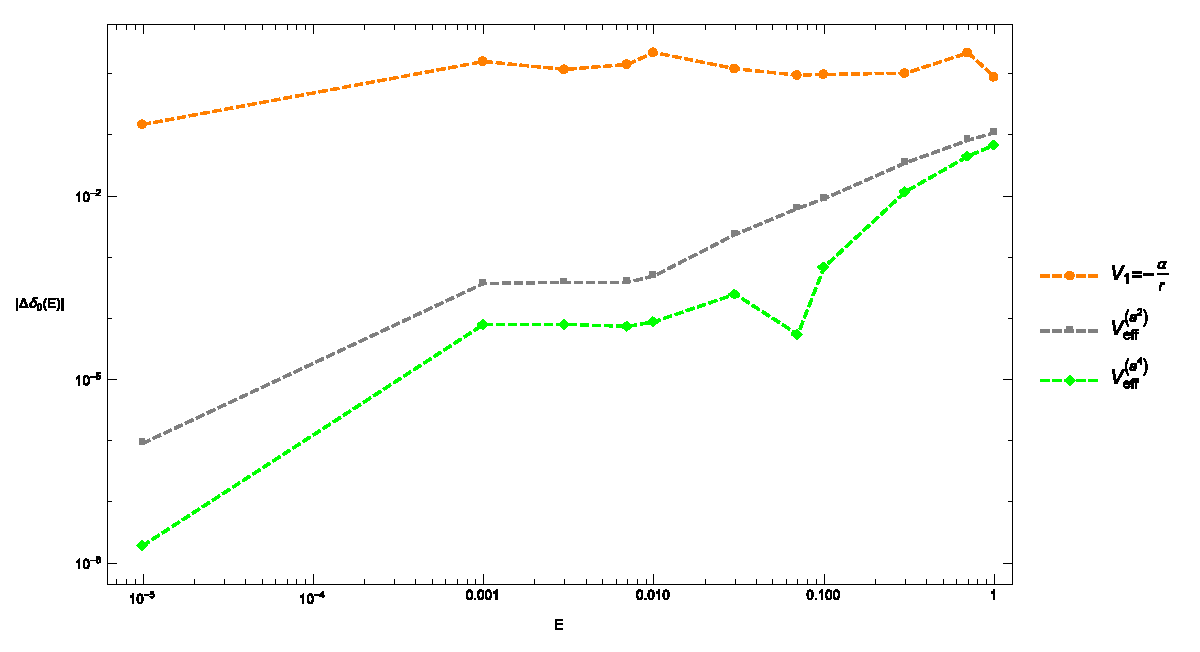
\includegraphics[width=4.3in]{Test_PS_CurveFitting_Figure3.eps}
	\caption{不同势对应相移的绝对误差}\label{Swavephaseerror}
\end{figure}
\end{frame}

%\begin{frame}
%\frametitle{截断$a$的影响}
%\begin{figure}[!tp]
%	\centering
%	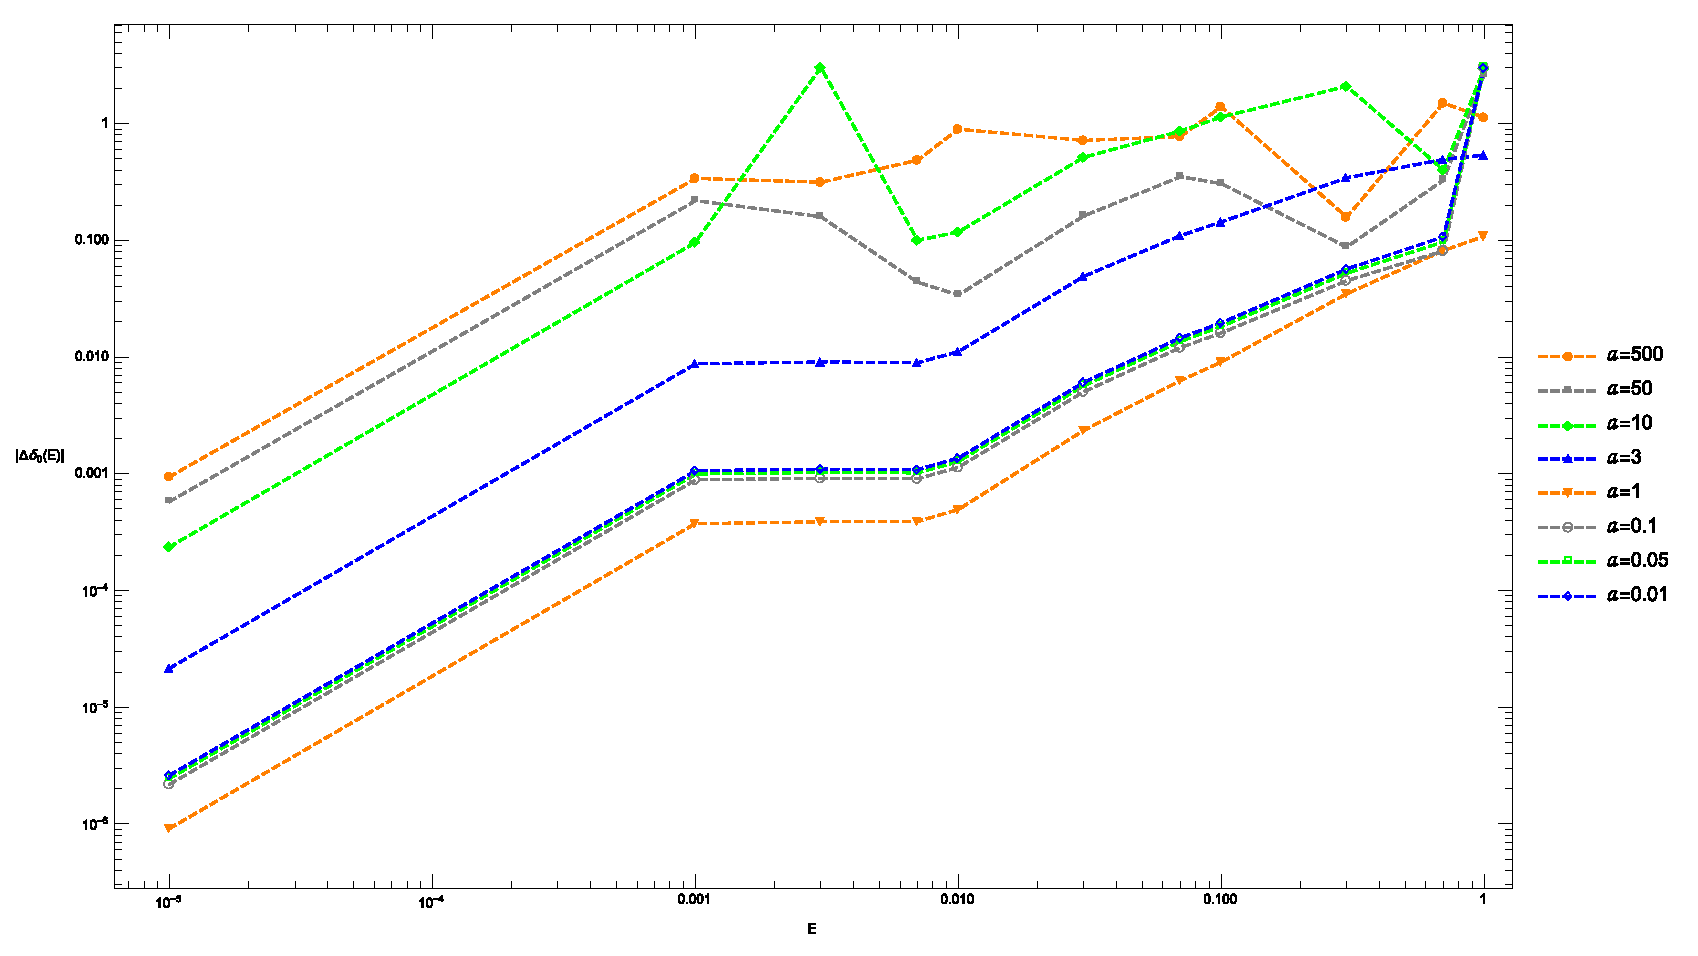
\includegraphics[width=4.2in]{Test_PhaseShift_Various_a.eps}
%	\caption{截断$a$的取值对有效势相移误差的影响}\label{cutoffa}
%\end{figure}
%\end{frame}
%
%\begin{frame}
%\begin{figure}[!htbp]
%	\begin{minipage}[t]{0.37\linewidth}
%		\centering
%		\includegraphics[width=1\textwidth]{{Test_Determine_a_Alpha=0.01&m=10}.eps}
%	\end{minipage}
%	\begin{minipage}[t]{0.37\linewidth}
%		\centering
%		\includegraphics[width=1\textwidth]{{Test_Determine_a_Alpha=0.1&m=1}.eps}
%	\end{minipage}\\
%
%	\begin{minipage}[t]{0.37\linewidth}
%		\centering
%		\includegraphics[width=1\textwidth]{{Test_Determine_a_Alpha=0.1&m=10}.eps}
%	\end{minipage}
%	\begin{minipage}[t]{0.37\linewidth}
%		\centering
%		\includegraphics[width=1\textwidth]{{Test_Determine_a_Alpha=0.01&m=100}.eps}
%	\end{minipage}\\
%
%	\begin{minipage}[t]{0.37\linewidth}
%		\centering
%		\includegraphics[width=1\textwidth]{{Test_Determine_a_Alpha=1&m=10}.eps}
%	\end{minipage}
%	\begin{minipage}[t]{0.37\linewidth}
%		\centering
%		\includegraphics[width=1\textwidth]{{Test_Determine_a_Alpha=0.1&m=100}.eps}
%	\end{minipage}
%	\caption{库伦势附加短程势时$a$的不同取值对有效势相移误差的影响}\label{diffa}
%\end{figure}
%\end{frame}
%
%\begin{frame}
%\begin{figure}[!tbp]
%	\begin{minipage}[t]{0.37\linewidth}
%		\centering
%		\includegraphics[width=1\textwidth]{{Test_Determine_Coulomb_a_Alpha=0.01&m=10}.eps}
%	\end{minipage}
%	\begin{minipage}[t]{0.37\linewidth}
%		\centering
%		\includegraphics[width=1\textwidth]{{Test_Determine_Coulomb_a_Alpha=0.1&m=1}.eps}
%	\end{minipage}\\
%
%	\begin{minipage}[t]{0.37\linewidth}
%		\centering
%		\includegraphics[width=1\textwidth]{{Test_Determine_Coulomb_a_Alpha=0.1&m=10}.eps}
%	\end{minipage}
%	\begin{minipage}[t]{0.37\linewidth}
%		\centering
%		\includegraphics[width=1\textwidth]{{Test_Determine_Coulomb_a_Alpha=0.01&m=100}.eps}
%	\end{minipage}\\
%
%	\begin{minipage}[t]{0.37\linewidth}
%		\centering
%		\includegraphics[width=1\textwidth]{{Test_Determine_Coulomb_a_Alpha=1&m=10}.eps}
%	\end{minipage}
%	\begin{minipage}[t]{0.37\linewidth}
%		\centering
%		\includegraphics[width=1\textwidth]{{Test_Determine_Coulomb_a_Alpha=0.1&m=100}.eps}
%	\end{minipage}
%	\caption{库伦势不附加短程势时$a$的不同取值对有效势相移误差的影响}\label{Coulombdiffa}
%\end{figure}
%\end{frame}

%\begin{frame}
%\frametitle{跑动耦合}
%研究有效势$V_{eff}^{(a^2)}$的耦合常数$c$对截断$a$的依赖:
%\begin{figure}[!hbtp]
%	\begin{minipage}[t]{0.329\linewidth}
%		\centering
%		\includegraphics[width=1\textwidth]{{Plot_c1_veus_a_Alpha=0.1&m=1}.eps}
%	\end{minipage}
%	\begin{minipage}[t]{0.329\linewidth}
%		\centering
%		\includegraphics[width=1\textwidth]{{Plot_c1_veus_a_Alpha=0.3&m=1}.eps}
%	\end{minipage}
%	\begin{minipage}[t]{0.329\linewidth}
%		\centering
%		\includegraphics[width=1\textwidth]{{Plot_c1_veus_a_Alpha=0.4&m=1}.eps}
%	\end{minipage}
%	%\caption{有效势$V_{eff}^{(a^2)}$的耦合常数$c$对截断$a$的依赖}\label{cveusa}
%\end{figure}
%当截断$a$的值发生变动的时候,我们所匹配的耦合常数$c$同时也会发生变化,类似地现象在场论中被称作跑动耦合。
%\end{frame}

\begin{frame}
\frametitle{矩阵元}
矩阵元不是物理可观测量,其体现了更多“真实”的短程结构,因此需要添加更多的修正项才能使得有效理论中的矩阵元能够和“真实”的矩阵元对应起来。以$\expval{\vb{p}^4}$为例:
\begin{table}[!hbtp]
\footnotesize
  \centering
  \begin{tabular}{|cccccc|}
    \hline
    % after \\: \hline or \cline{col1-col2} \cline{col3-col4} ...
    能级 & $\expval{\vb{p}^4}$ & $\expval{\vb{p^4}}_{eff}$ & $\expval{\vb{p^4}}_{eff}$相对误差 & $\expval{Z\vb{p}^4+\gamma \delta^3_a/a+\dots}_{eff}$ & 修正后相对误差 \\
    \hline
    1S & 75.0651 & 6.39016&0.914872 & 86.2584&0.149114 \\
    2S & 5.89805 & 1.80467&0.694022 & 5.63427&0.0447230 \\
    3S & 1.38388 & 0.459182&0.668193 & 1.37834&0.00400119 \\
    4S & 0.533537 & 0.181115&0.660539 & 0.533006&0.000995149 \\
    5S & 0.259685 & 0.0892336&0.656377 & 0.259594&0.000349898 \\
    6S & 0.145438 & 0.0503636&0.653711 & 0.145417&0.000142768 \\
    10S& 0.0294762 & 0.0103588 & 0.648572 & 0.0294762 & $0.\times10^{-50}$\\
    15S& 0.00846592 & 0.00299626 & 0.646080 & 0.00846592 &  $0.\times10^{-50}$\\
    20S& 0.00503698 & 0.00278627 & 0.446837 & 0.00503698 & $0.\times10^{-50}$\\
    \hline
  \end{tabular}
  \caption{$\expval{\vb{p}^4}$矩阵元在真实势及有效理论(相移)中的对比}\label{p41}
\end{table}
我们还对$\displaystyle\expval{\frac{1}{r}}$、$\displaystyle\expval{\frac{1}{r^2}}$、$\displaystyle\expval{r}$、$\displaystyle\expval{e^{-r}}$矩阵元进行了相似地计算。
\end{frame}

\begin{frame}
\frametitle{矩阵元的修正}
\begin{itemize}
\item 为使有效理论中的矩阵元能够与“真实”矩阵元相匹配,我们需要对其进行修正:
\begin{equation}\label{p4true}
	\expval{\vb{p}^4}_{true}=Z\expval{\vb{p^4}}_{eff}+\frac{\gamma}{a}\expval{\delta^3_a(\vb{r})}_{eff}+\eta a\expval{\laplacian{\delta^3_a(\vb{r})}}_{eff}+\mathcal{O}(a^3)
\end{equation}
上式共有$Z$、$\gamma$、$\eta$三个无量纲的参数待定,我们需要利用“真实”矩阵元的相应匹配来得到这些参数的值。

\vspace{12pt}
\item 选择10S、15S与20S能级的$\expval{\vb{p}^4}$“真实”矩阵元进行匹配,我们得到$Z=1.26946$、$\gamma=1243.77$与$\eta=82.2527$。

\vspace{12pt}
\item 这一关系对其它的矩阵元同样适用,应用上式我们可以得到较精确的结果。
\vspace{12pt}
\item 类似于算符乘积展开
\end{itemize}
\end{frame}

\begin{frame}
\frametitle{波函数}
\begin{itemize}
  \item 零点波函数
  \begin{equation}\label{psi0}
	\psi_{true}(0)=\overline{\gamma}\int\dd^3r\psi_{eff}\delta^3_a(\vb{r})+\overline{\eta}a^2\int\dd^3r\psi_{eff}\laplacian{\delta^3_a(\vb{r})}+\mathcal{O}(a^3)
\end{equation}
  \item 完整波函数
  \begin{equation}\label{psi0r}
	\psi_{true}(r<a)=\overline{\gamma}(r)\int\dd^3r\psi_{eff}\delta^3_a(\vb{r})+\overline{\eta}(r)a^2\int\dd^3r\psi_{eff}\laplacian{\delta^3_a(\vb{r})}+\mathcal{O}(a^3)
\end{equation}
\item 二阶导数
\begin{alignat}{1}\label{psi0rl}
	\laplacian{\psi_{true}(r)}= & \overline{\gamma}(r)\int\dd^3r\psi_{eff}\delta^3_a(\vb{r})+\overline{\gamma'}(r)\int\dd^3r\laplacian{\bqty{\psi_{eff}\delta^3_a(\vb{r})}}+\overline{\eta}(r)a^2\int\dd^3r\psi_{eff}\laplacian{\delta^3_a(\vb{r})}
	\nonumber\\\nonumber+&\overline{\eta'}(r)a^2\int\dd^3r\laplacian{\bqty{\psi_{eff}\laplacian{\delta^3_a(\vb{r})}}}+\mathcal{O}(a^3)\\
=&\overline{\gamma}(r)\int\dd^3r\psi_{eff}\delta^3_a(\vb{r})+\overline{\eta}(r)a^2\int\dd^3r\psi_{eff}\laplacian{\delta^3_a(\vb{r})}+\mathcal{O}(a^3)
\end{alignat}
\end{itemize}
\end{frame}

\begin{frame}
\begin{figure}[!htbp]
	\centering
	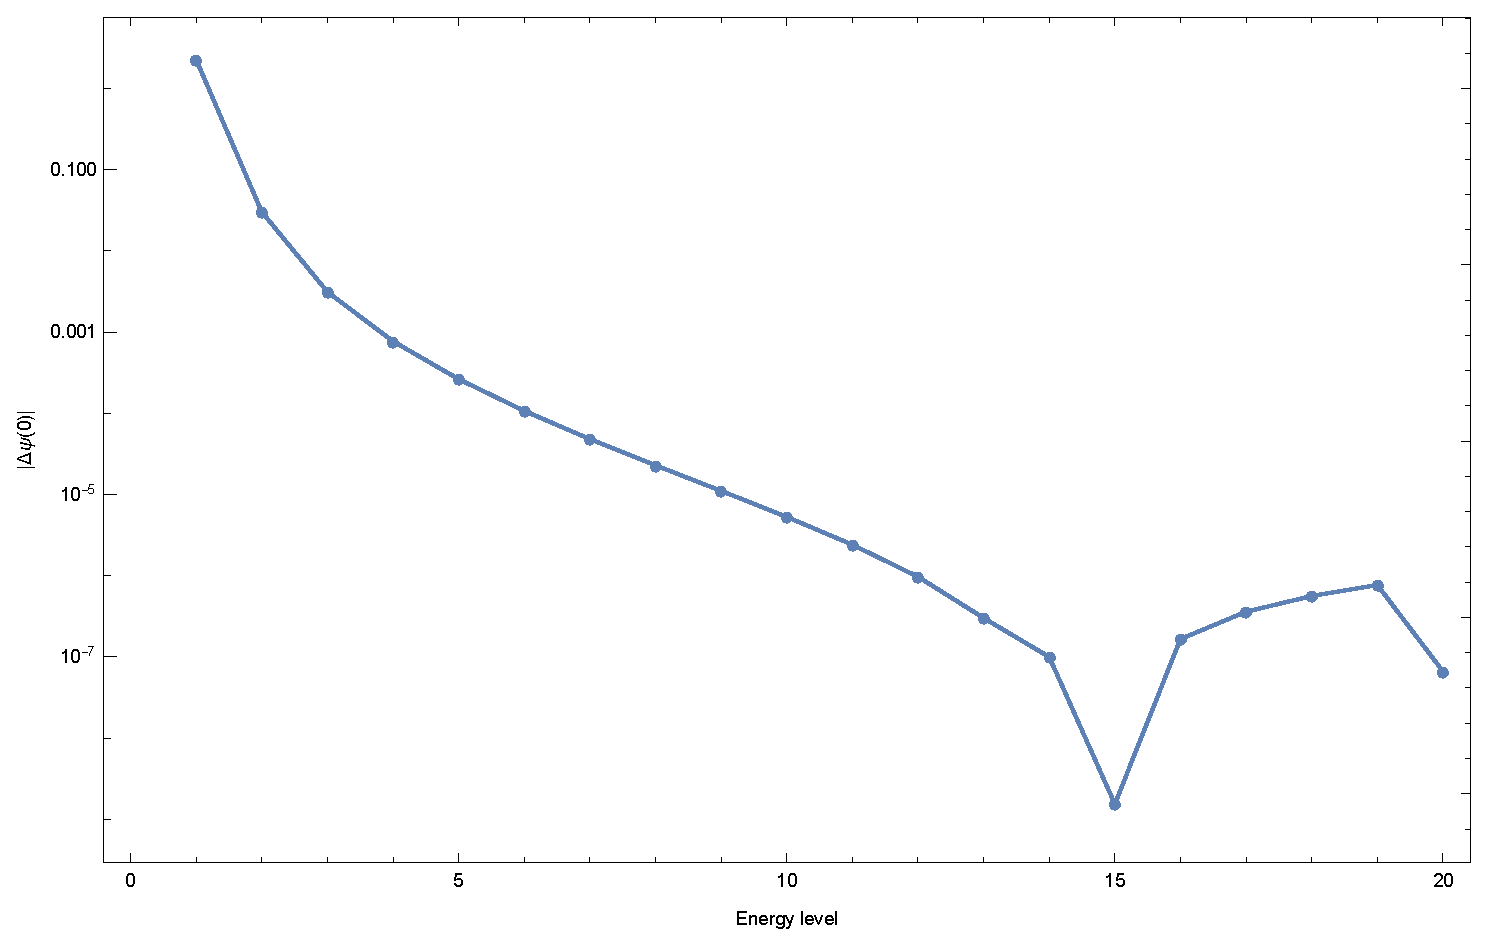
\includegraphics[width=4.3in]{psir1.eps}
	\caption{$\psi_{true}(r)$($r\leq a$)各能级相对于“真实”波函数的相对误差}\label{psir}
\end{figure}
\end{frame}
%
%\begin{frame}
%\frametitle{其它势的有效理论\footnote{我们总共计算了5种不同的短程势组合,另外两种分别为$c \frac{e^{-dr}}{r}$与$e \frac{e^{-fr^2}}{r}$。对于另外两种短程势,我们发现其紫外发散行为与库伦势本身十分接近,因此并未列出。}}
%\begin{itemize}
%\item 库伦势
%\vspace{12pt}
%\item	$\displaystyle V_1=-\frac{\alpha}{r}+\begin{cases}
%	a, & \mbox{if } 0\leq r<1 \\
%	0, & \mbox{otherwise}.
%	\end{cases}$
%%	V_2&=&-\frac{\alpha}{r}+c \frac{e^{-dr}}{r}\\
%%	V_3&=&-\frac{\alpha}{r}+e \frac{e^{-fr^2}}{r}\\
%%	V_4&=&-\frac{\alpha}{r}+g e^{-hr}\\
%%	V_5&=&-\frac{\alpha}{r}+je^{-kr^2}
%\vspace{12pt}
%\item	$\displaystyle V_2=-\frac{\alpha}{r}+g e^{-hr}$
%\vspace{12pt}
%\item	$\displaystyle V_3=-\frac{\alpha}{r}+je^{-kr^2}$
%\end{itemize}
%
%\end{frame}

\section{常见误解}
\begin{frame}
\frametitle{常见误解}
\begin{itemize}
  \item 构建出的有效理论随着修正项的添加而渐渐成为真实物理
  \vspace{12pt}
  \item 当动量$q\ll\Lambda=\displaystyle\frac{1}{a}$时,动量空间中的有效势将会逐渐接近“真实”势,并最终在$q\rightarrow0$时收敛到“真实”势
  \vspace{12pt}
  \item 有效理论只是简单的拟合方法,添加的项数越多,参数越多,结果也就越精确
\end{itemize}

\end{frame}

\begin{frame}
\frametitle{构建出的有效理论随着修正项的添加而渐渐成为真实物理}
\footnotesize
\begin{eqnarray}\label{realpo}
	% \nonumber % Remove numbering (before each equation)
	V(\vb{r}) &=& -\frac{1}{r}-\frac{1.04152 e^{-0.9991 r}}{r} \\
	\label{effa2} V_{eff}^{(a^2)}(\vb{r}) &=& -\frac{\text{erf}\left(\frac{r}{\sqrt{2}}\right)}{r}-2.81241 e^{-\frac{r^2}{2}} \\
	\label{effa4} V_{eff}^{(a^4)}(\vb{r}) &=& -\frac{\text{erf}\left(\frac{r}{\sqrt{2}}\right)}{r}-2.53643 e^{-\frac{r^2}{2}}+3.26552 \left(\frac{e^{-\frac{r^2}{2}} r^2}{2 \sqrt{2} \pi ^{3/2}}-\frac{3 e^{-\frac{r^2}{2}}}{2 \sqrt{2} \pi ^{3/2}}\right)
\end{eqnarray}
\begin{figure}[!hbp]
	\centering
	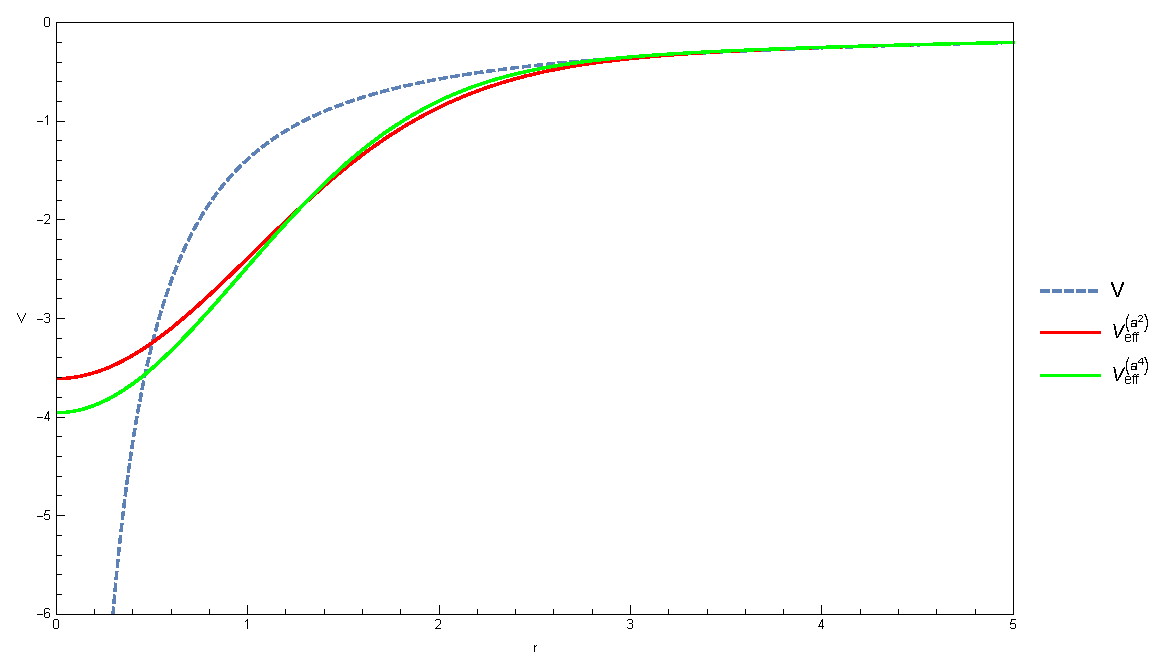
\includegraphics[width=2.8in]{NoFourierTransformation.eps}
%	\caption{有效势与真实势在坐标空间的对比}\label{nofourier}
\end{figure}
\end{frame}

\begin{frame}
\frametitle{动量$q\ll\Lambda=\displaystyle\frac{1}{a}$时,动量空间中的有效势将趋于“真实”势}
\footnotesize
\begin{eqnarray}
	% \nonumber % Remove numbering (before each equation)
	v(\vb{k}) &=& -\frac{4 \pi }{k^2}-\frac{13.0882}{k^2+0.998201} \\
	v_{eff}^{(a^2)}(\vb{k}) &=& -\frac{4 \pi }{k^2}\; e^{-\frac{k^2}{2}}-44.2944\; e^{-\frac{k^2}{2}} \\
	v_{eff}^{(a^4)}(\vb{k}) &=& -\frac{4 \pi  }{k^2}\;e^{-\frac{k^2}{2}}-\left(3.26552 k^2+39.9477\right)e^{-\frac{k^2}{2}}
\end{eqnarray}
\begin{figure}[!hbp]
	\centering
	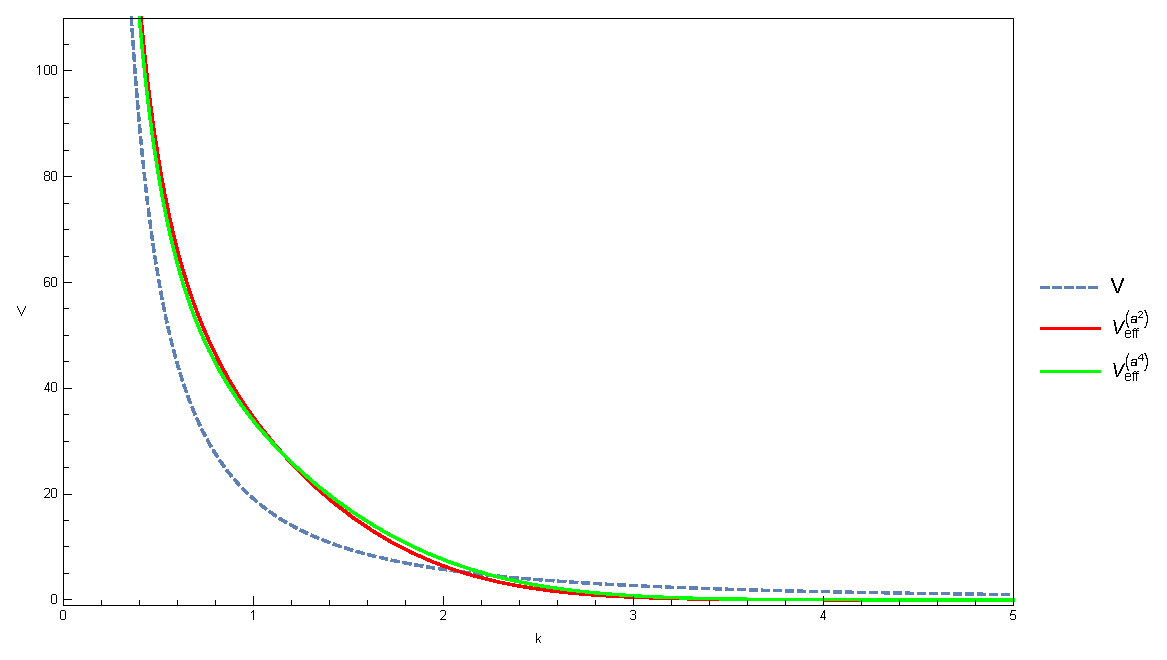
\includegraphics[width=2.8in]{FourierTransformation_1.eps}
	\caption{有效势与真实势在动量空间的对比}\label{TotalFourier}
\end{figure}
\end{frame}

\begin{frame}
\begin{figure}[!bp]
\begin{minipage}[t]{0.45\linewidth}
	\centering
	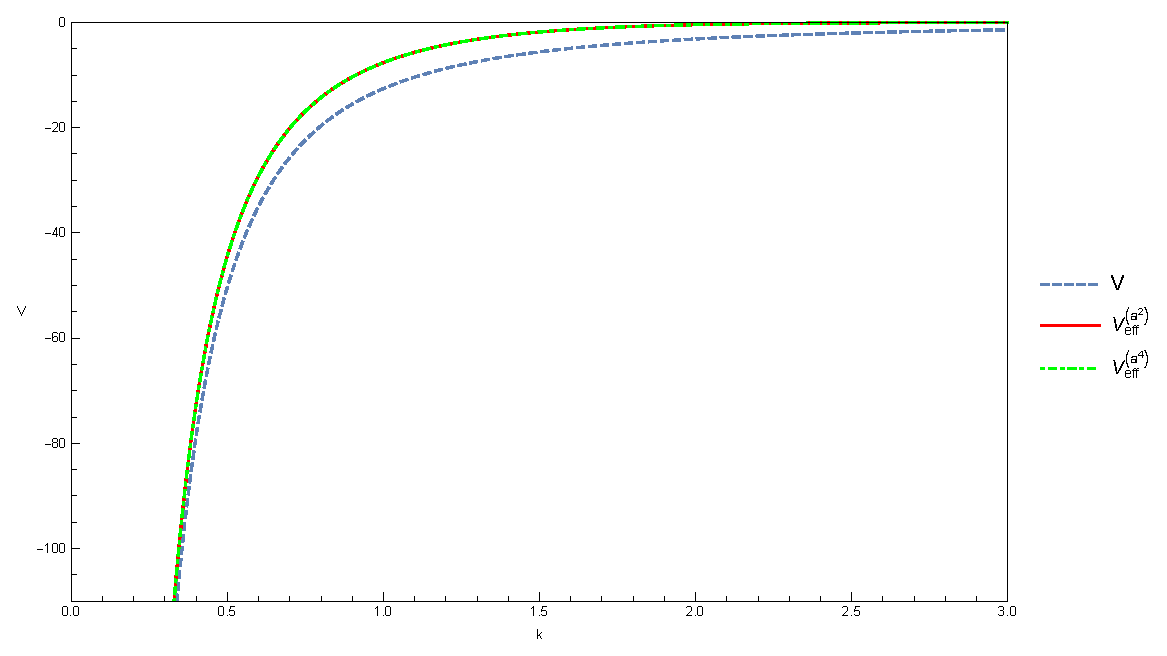
\includegraphics[width=\textwidth]{FourierTransformation_2.eps}
	\caption{有效势与真实势函数动量空间函数的第一项对比}\label{fourpart1}
\end{minipage}
\begin{minipage}[t]{0.45\linewidth}
	\centering
	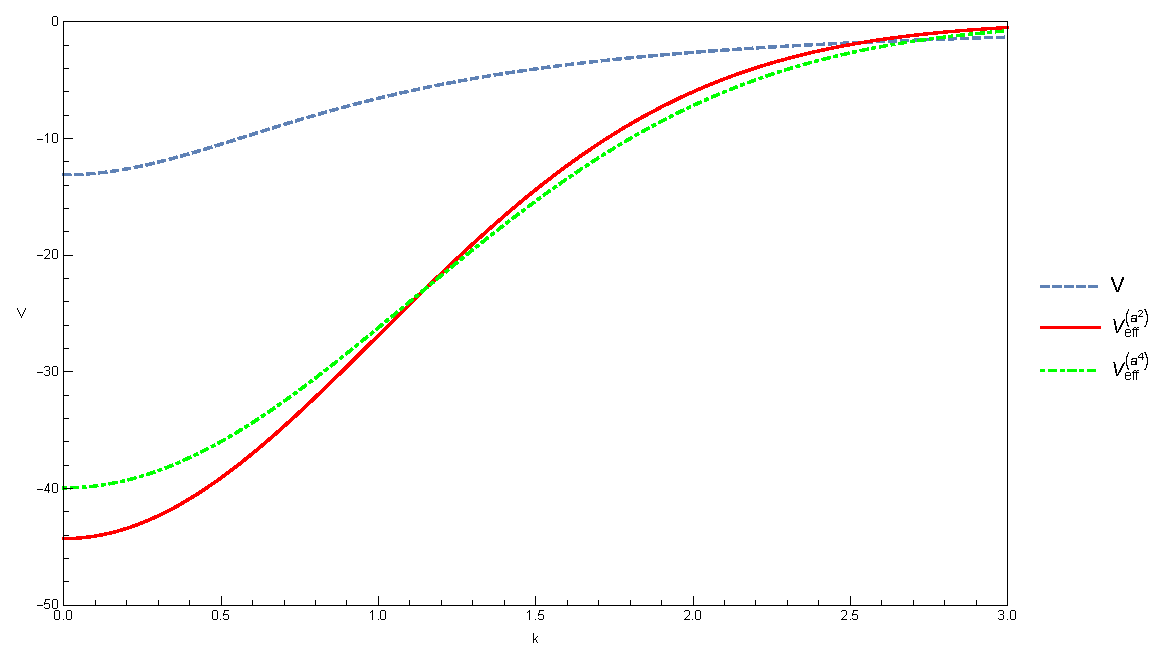
\includegraphics[width=\textwidth]{FourierTransformation_3.eps}
	\caption{有效势与真实势动量空间函数的剩余项对比}\label{fourpart2}
\end{minipage}
\begin{minipage}[t]{0.45\linewidth}
\centering
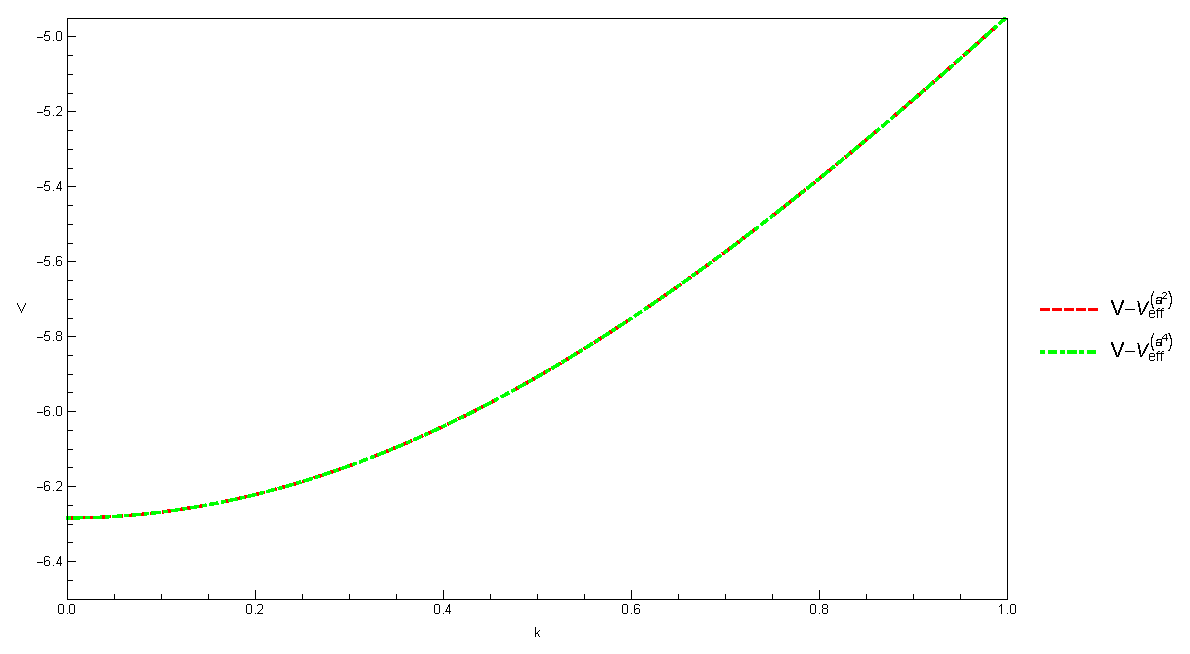
\includegraphics[width=\textwidth]{FourierTransformation_4.eps}
\caption{真实势与有效势动量空间函数第一项的差值}\label{fourminus}
\end{minipage}
\end{figure}
\end{frame}

\begin{frame}
\frametitle{有效理论只是简单的拟合方法}
\begin{itemize}
  \item 构建有效理论时大量用到了曲线拟合(参数匹配)的方法
  \vspace{12pt}
  \item 添加的项数越多,参数越多,结果也就越精确
  \vspace{12pt}
  \item 更加系统化,误差项随着$a$阶数的升高而逐项移除
  \vspace{12pt}
  \item 遵循重整化理论的思想,确定修正项的形式以及可以调节的参数(在场论中即是耦合常数)的数量、位置
\end{itemize}
\end{frame}
%
%\section{有效理论的微扰匹配}
%\begin{frame}
%\frametitle{有效理论的微扰匹配}
%\begin{itemize}
%\item 对库伦势的有效理论,我们有
%\begin{equation}\label{CoulombSmall}
%	H_{eff}=\frac{\vb{p}^2}{2m}-\frac{\alpha}{r}\text{erf}(\frac{r}{\sqrt{2}a})-2\pi\alpha ca^2\delta_a^3(\vb{r})
%\end{equation}
%\item 可使用微扰方法来确定参数$c$的值
%\item 利用玻恩近似得到散射振幅并进行匹配
%\item 例如,利用一级玻恩近似确定参数$c$的值:对$H$,有
%\begin{equation}
%	f^{(1)}(\vb{q})=\int\dd^3 x' e^{-i\vb{q}\cdot\vb{x'}}V=-\frac{4\pi\alpha}{q^2}
%\end{equation}
%其中$\vb{q}=\vb{k_0}-\vb{k'}$为动量转移。而对$H_{eff}$,有
%\begin{eqnarray}\label{Heff}
%	\nonumber f_{eff}^{(1)}(\vb{q})&=&-\frac{4\pi\alpha}{q^2}e^{-q^2a^2/2}(1+cq^2a^2/2)\\
%	&=&-\frac{4\pi\alpha}{q^2}(1+(c-1)q^2a^2/2+\mathcal{O}(q^4a^4))
%\end{eqnarray}
%\end{itemize}
%\end{frame}

\section{结论}
\begin{frame}
\frametitle{结论}
\begin{itemize}
  \item 有效理论对物理可观测量的计算能够达到较高精度,并且精度随能量减小而增加;当能量达到一定上限后,有效理论即失去作用,误差变得极大。
  \vspace{12pt}
  \item 仅有物理可观测量在有效理论中可以与真实物理量符合较好,而其他非物理的量则不然;但是我们可以添加额外的修正项来弥补矩阵元等所体现的“真实”物理的短程结构;在添加修正项后,矩阵元等的精度也有了较大的提升。
  \vspace{12pt}
  \item 可以利用微扰匹配方法得到有效理论中的耦合常数
  \vspace{12pt}
  \item 有效理论的可行性与真实物理的具体形式无关
\end{itemize}

\end{frame}

%\begin{frame}
%\frametitle{致谢}
%
%\end{frame}

\begin{frame}
  \Huge
	\begin{center}
	Thank you!
	\end{center}
\end{frame}

\end{document}
